\documentclass[]{article}
\usepackage{lmodern}
\usepackage{amssymb,amsmath}
\usepackage{ifxetex,ifluatex}
\usepackage{fixltx2e} % provides \textsubscript
\ifnum 0\ifxetex 1\fi\ifluatex 1\fi=0 % if pdftex
  \usepackage[T1]{fontenc}
  \usepackage[utf8]{inputenc}
\else % if luatex or xelatex
  \ifxetex
    \usepackage{mathspec}
    \usepackage{xltxtra,xunicode}
  \else
    \usepackage{fontspec}
  \fi
  \defaultfontfeatures{Mapping=tex-text,Scale=MatchLowercase}
  \newcommand{\euro}{€}
\fi
% use upquote if available, for straight quotes in verbatim environments
\IfFileExists{upquote.sty}{\usepackage{upquote}}{}
% use microtype if available
\IfFileExists{microtype.sty}{%
\usepackage{microtype}
\UseMicrotypeSet[protrusion]{basicmath} % disable protrusion for tt fonts
}{}
\usepackage[margin=1in]{geometry}
\usepackage{longtable,booktabs}
\usepackage{graphicx}
\makeatletter
\def\maxwidth{\ifdim\Gin@nat@width>\linewidth\linewidth\else\Gin@nat@width\fi}
\def\maxheight{\ifdim\Gin@nat@height>\textheight\textheight\else\Gin@nat@height\fi}
\makeatother
% Scale images if necessary, so that they will not overflow the page
% margins by default, and it is still possible to overwrite the defaults
% using explicit options in \includegraphics[width, height, ...]{}
\setkeys{Gin}{width=\maxwidth,height=\maxheight,keepaspectratio}
\ifxetex
  \usepackage[setpagesize=false, % page size defined by xetex
              unicode=false, % unicode breaks when used with xetex
              xetex]{hyperref}
\else
  \usepackage[unicode=true]{hyperref}
\fi
\hypersetup{breaklinks=true,
            bookmarks=true,
            pdfauthor={RESURAL (JcB)},
            pdftitle={Activité des structures d'urgences : panorama 2014 de la région ALSACE},
            colorlinks=true,
            citecolor=blue,
            urlcolor=blue,
            linkcolor=magenta,
            pdfborder={0 0 0}}
\urlstyle{same}  % don't use monospace font for urls
\setlength{\parindent}{0pt}
\setlength{\parskip}{6pt plus 2pt minus 1pt}
\setlength{\emergencystretch}{3em}  % prevent overfull lines
\setcounter{secnumdepth}{5}

%%% Use protect on footnotes to avoid problems with footnotes in titles
\let\rmarkdownfootnote\footnote%
\def\footnote{\protect\rmarkdownfootnote}

%%% Change title format to be more compact
\usepackage{titling}

% Create subtitle command for use in maketitle
\newcommand{\subtitle}[1]{
  \posttitle{
    \begin{center}\large#1\end{center}
    }
}

\setlength{\droptitle}{-2em}
  \title{Activité des structures d'urgences : panorama 2014 de la région ALSACE}
  \pretitle{\vspace{\droptitle}\centering\huge}
  \posttitle{\par}
  \author{RESURAL (JcB)}
  \preauthor{\centering\large\emph}
  \postauthor{\par}
  \predate{\centering\large\emph}
  \postdate{\par}
  \date{28/01/2015}



\begin{document}

\maketitle


{
\hypersetup{linkcolor=black}
\setcounter{tocdepth}{3}
\tableofcontents
}
Version mse à jour le: \textbf{Thu Aug 20 19:12:02 2015}

Ajout de la dernière version de Gilles

\begin{itemize}
\itemsep1pt\parskip0pt\parsep0pt
\item
  nombre de passages pour 10.000 hab.
\item
  nombre de SU pour 10.000 hab.
\item
  nombre de lignes SMUR financées par une MIG
\item
  nombre de siège de SMUR dont SMUR saisonnier dont antenne SMUR dont
  hélismur
\item
  séparer privés lucratifs et ESPIC
\item
  nombre de logicels et nombre de SU par région
\item
  SAE 2014 ?
\item
  augmentation par rapport année N-1 en tenant compte uniquement des
  établissements ``stables''
\item
  séparer chu et non chu, samu de chu et de non chu
\item
  retour attendu pour le 4/9
\end{itemize}

\section{Activité des structures d'urgences : panorama 2014 de la région
ALSACE}\label{activite-des-structures-durgences-panorama-2014-de-la-region-alsace}

Rapport 2014 respectant les préconisations de la FEDORU. Source:
\href{https://docs.google.com/document/d/101LYVqVLeHZnrujfMm3aqBYfbOwx3CPEB3Y-Lbud2Ls/edit}{Trame
commune}

Le document de référence pour le rapport est: \textbf{V4 trame commune
2014 rapport inter région} (xps:
/home/jcb/Documents/Resural/FEDORU/Trame\_Commune/DOC/Trame commune 2014
rapport inter région (V4).docx)

\textbf{NOTE}: certaines informations utiles sont dans
\textbf{RPU\_Doc}.

\section{LE MOT DU PRÉSIDENT DE LA
FEDORU}\label{le-mot-du-president-de-la-fedoru}

La publication du panorama des urgences de la région
\textbf{ALSACE}constitue une excellente occasion pour présenter la
fédération des observatoires régionaux des urgences (FEDORU) qui compte
\textbf{RESURAL} parmi ses membres actifs.

La FEDORU a été créée au mois d'octobre 2013. Ses membres sont chargés
dans leur région respective du traitement des données d'urgences ; ce
point commun est le trait d'origine de la FEDORU et donne son empreinte
à l'objet de notre association que je cite ici :

\begin{itemize}
\itemsep1pt\parskip0pt\parsep0pt
\item
  promouvoir les observatoires régionaux des urgences et les structures
  ayant une activité similaire ;
\item
  promouvoir toutes les actions visant à améliorer la connaissance sur
  les soins de premier recours ;
\item
  partager les expertises dans le domaine du recueil, de l'analyse et de
  l'évaluation de la qualité des données relatives à l'activité des
  urgences.
\end{itemize}

Les premières publications de la FEDORU (disponibles sur le site :
\url{http://www.fedoru.fr}) abordent les thèmes techniques suivants :

\begin{itemize}
\itemsep1pt\parskip0pt\parsep0pt
\item
  Recommandations pour la création d'un ORU
\item
  Collecte et usage des RPU
\item
  Hôpital en tension - Synthèse FEDORU
\end{itemize}

Ces documents constituent le socle indispensable à la conduite de
travaux inter-régionaux. Nous pourrons ainsi comparer nos résultats,
harmoniser les indicateurs retenus dans nos publications respectives,
travailler sur des échantillons de données plus importants(inter-région
ou national), mais aussi évaluer l'impact de différentes organisations.

La recherche de consensus et d'échanges entre les différents acteurs
régionaux représentés au sein de la FEDORU s'illustre parfaitement dans
cette publication qui prend le parti de respecter les premières
recommandations sur le traitement des RPU. Le ``panorama des urgences en
région \ldots{}.'', intègre le format d'analyse commun 2015 proposé de
manière collégiale par nos groupes experts et validé par notre conseil
d'administration. Ce socle d'analyse produit par ``la structure
concernée'' sera rapproché des résultats des autres régions et donnera
lieu à une publication commune au cours de l'année 2015. J'adresse au
nom de la FEDORU toutes mes félicitations à l'ensemble de l'équipe de
\textbf{RESURAL} pour la qualité de leurs travaux mais aussi et surtout
à tous les professionnels des services d'urgences de l'\textbf{ALSACE}
pour le fastidieux mais si précieux travail de collecte sur le terrain.

\textbf{Dr G. VIUDES}

\emph{Président de la FEDORU}

\section{Description de l'offre de
soins}\label{description-de-loffre-de-soins}

\subsection{Qualité des données}\label{qualite-des-donnees}

Réalisation d'un diagramme radar présentant l'exhaustivité des items
RPU.

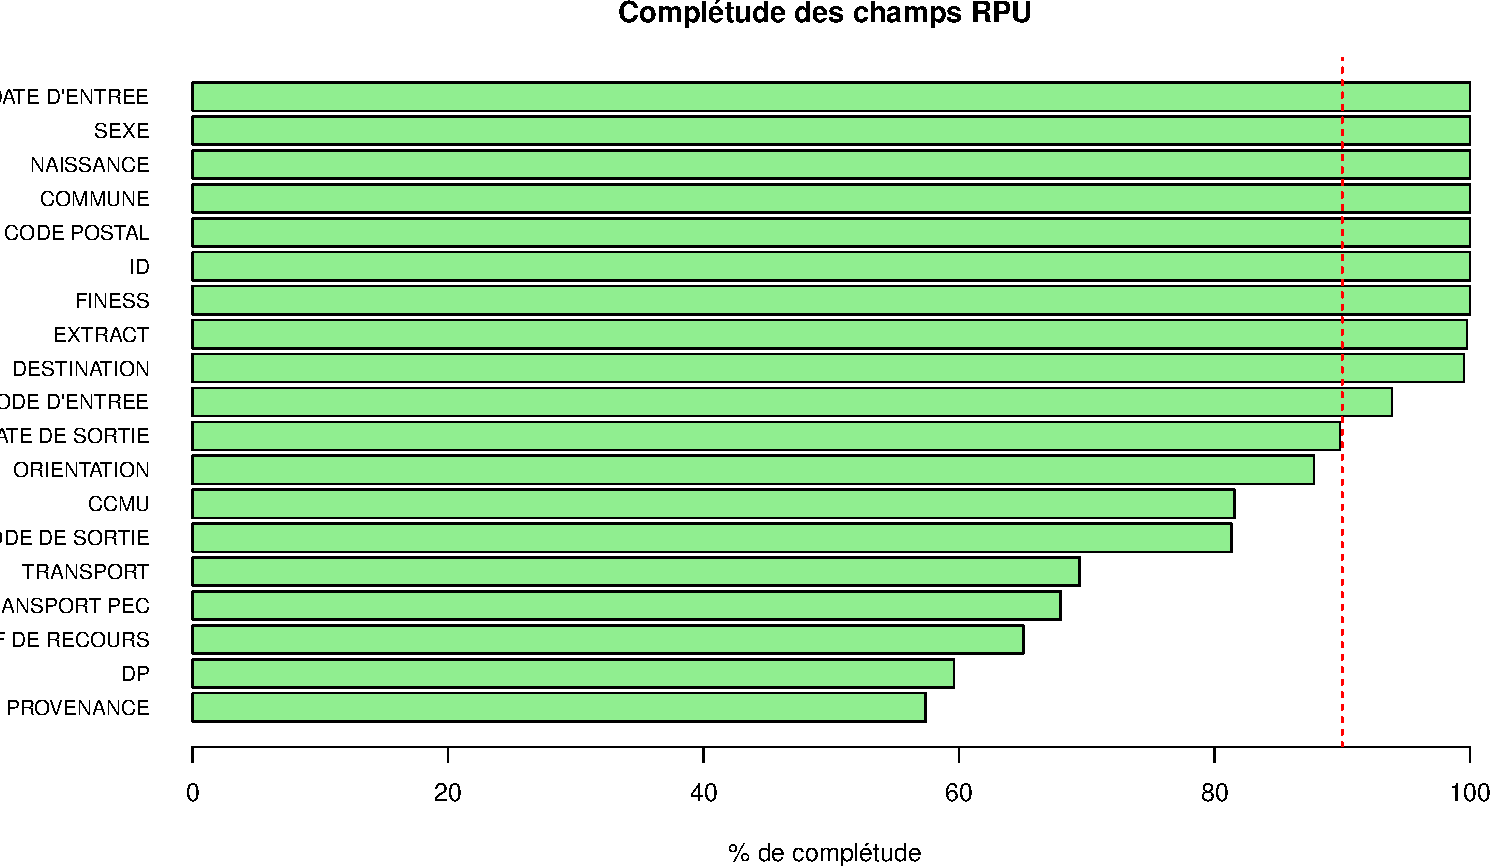
\includegraphics{rapport2014_V4_files/figure-latex/completude-1.pdf}
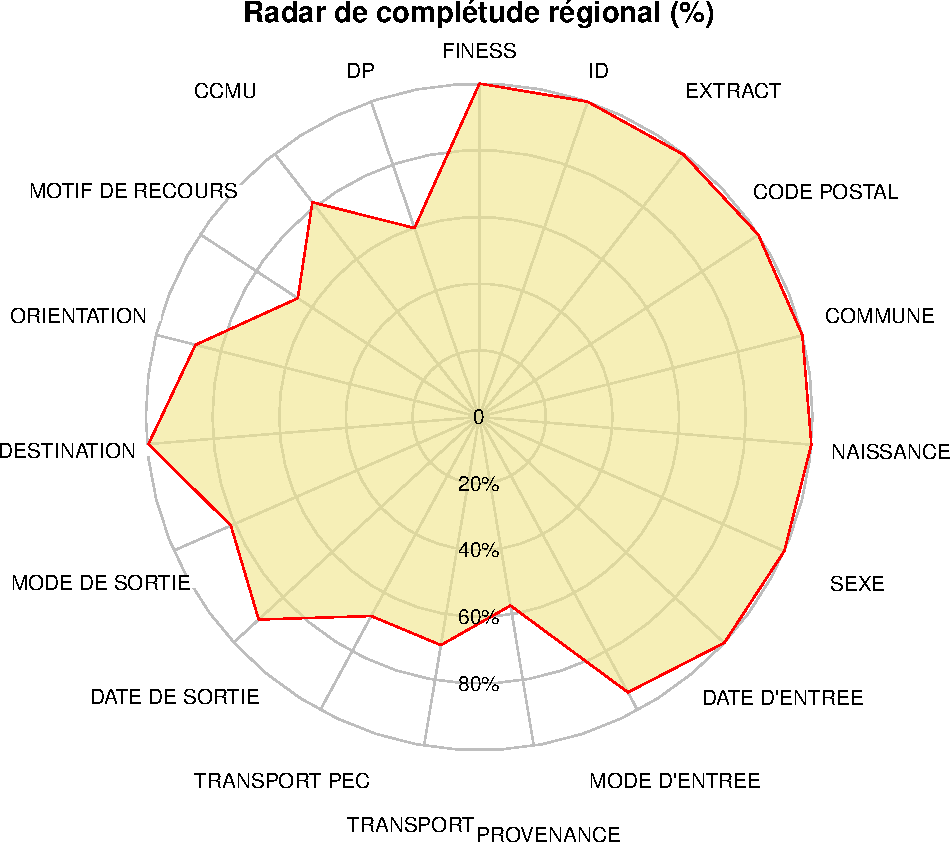
\includegraphics{rapport2014_V4_files/figure-latex/completude-2.pdf}

Complétude en valeur absolue et en pourcentages:`

\begin{verbatim}
##           FINESS               ID          EXTRACT      CODE POSTAL 
##           416733           416733           415731           416733 
##          COMMUNE        NAISSANCE             SEXE    DATE D'ENTREE 
##           416716           416733           416733           416733 
##    MODE D'ENTREE       PROVENANCE        TRANSPORT    TRANSPORT PEC 
##           391370           239122           289308           283189 
##   DATE DE SORTIE   MODE DE SORTIE      DESTINATION      ORIENTATION 
##           374349           338878            82635            72898 
## MOTIF DE RECOURS             CCMU               DP 
##           270962           339827           245974
\end{verbatim}

\begin{verbatim}
##           FINESS               ID          EXTRACT      CODE POSTAL 
##              100              100              100              100 
##          COMMUNE        NAISSANCE             SEXE    DATE D'ENTREE 
##              100              100              100              100 
##    MODE D'ENTREE       PROVENANCE        TRANSPORT    TRANSPORT PEC 
##               94               57               69               68 
##   DATE DE SORTIE   MODE DE SORTIE      DESTINATION      ORIENTATION 
##               90               81              100               88 
## MOTIF DE RECOURS             CCMU               DP 
##               65               82               60
\end{verbatim}

\section{Les chiffres clés de l'activité des services
d'urgences}\label{les-chiffres-cles-de-lactivite-des-services-durgences}

Le format des chiffres clés est celui défini par la FEDORU. Il est
commun à toutes les régions membres de la FEDORU.

\subsection{Recueil des données}\label{recueil-des-donnees}

\begin{itemize}
\itemsep1pt\parskip0pt\parsep0pt
\item
  Nombre de passages dans l'année: 432 170 (données SAE 2014)
\item
  Nombre de RPU déclarés: \textbf{416 733 RPU}
\item
  Exhaustivité du recueil: \textbf{96.43 \%}
\item
  Moyenne quotidienne de passages: \textbf{1 142 RPU/jour}
\item
  \%(N) d'évolution par rapport à année 2013: \textbf{22 \%}.
\item
  \% d'évolution moyenne sur les 5 dernières années (méthode calcul :
  \emph{pas de données disponibles}.
\item
  Données renseignées (données à partir desquelles tout le reste de
  l'analyse sera effectuée) = Nombre de RPU transmis: 416 733 RPU
\end{itemize}

\subsection{PATIENTS}\label{patients}

\subsubsection{Sexe}\label{sexe}

\begin{itemize}
\itemsep1pt\parskip0pt\parsep0pt
\item
  \%(N) Femme: 47.78 \% (217 617)
\item
  \%(N) Homme: 52.22 \% (199 110)
\item
  Sex ratio: \textbf{1.09}
\item
  Taux de masculinité: 0.52
\end{itemize}

\subsubsection{Age}\label{age}

\begin{itemize}
\item
  age moyen: \textbf{38 ans}.
\item
  age moyen des hommes: 35.9 ans.
\item
  age moyen des femmes: 40.3 ans.
\item
  \% (N) \textless{} 1 an: 15 376 (\textbf{3.69 \%})
\item
  \%(N) \textless{} 15 ans: 103 413 (\textbf{NA \%})
\item
  \%(N) \textless{} 18 ans: 119 213 (\textbf{28.61 \%})
\item
  \%(N) \textgreater{}= 75 ans: 57 271 (\textbf{13.74 \%})
\item
  Pyramide des ages:
\end{itemize}

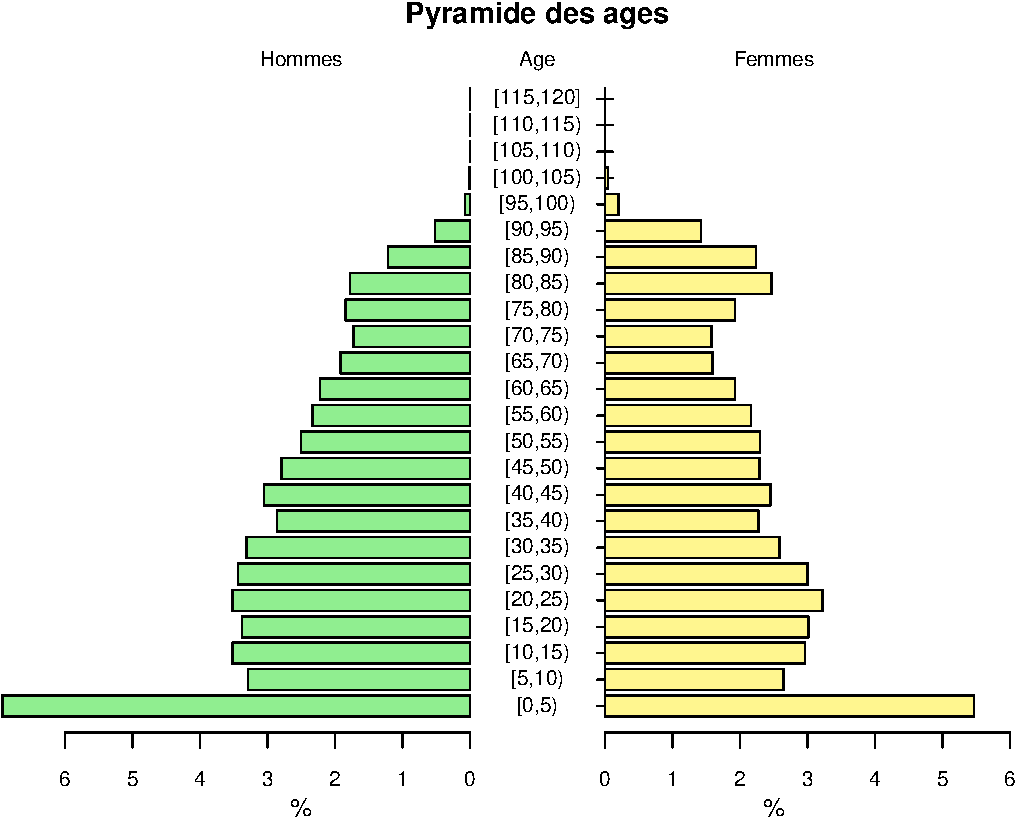
\includegraphics{rapport2014_V4_files/figure-latex/pyramide-1.pdf}

\begin{verbatim}
## [1] 5.1 4.1 4.1 2.1
\end{verbatim}

\subsubsection{Taux de recours (définition FEDORU) régional aux
urgences.}\label{taux-de-recours-definition-fedoru-regional-aux-urgences.}

Le taux de recours régional est calculé à partir des données de l'INSEE.

TARRU: \textbf{21.31\%} (ref: population alsacienne 2014)

\subsubsection{Pourcentage de patients ne venant pas de la région
(étranger
compris)}\label{pourcentage-de-patients-ne-venant-pas-de-la-region-etranger-compris}

Part des non résidents: \textbf{4.43\%} (N = 18467)

\subsection{ARRIVÉE}\label{arrivee}

\subsubsection{Horaires de passage}\label{horaires-de-passage}

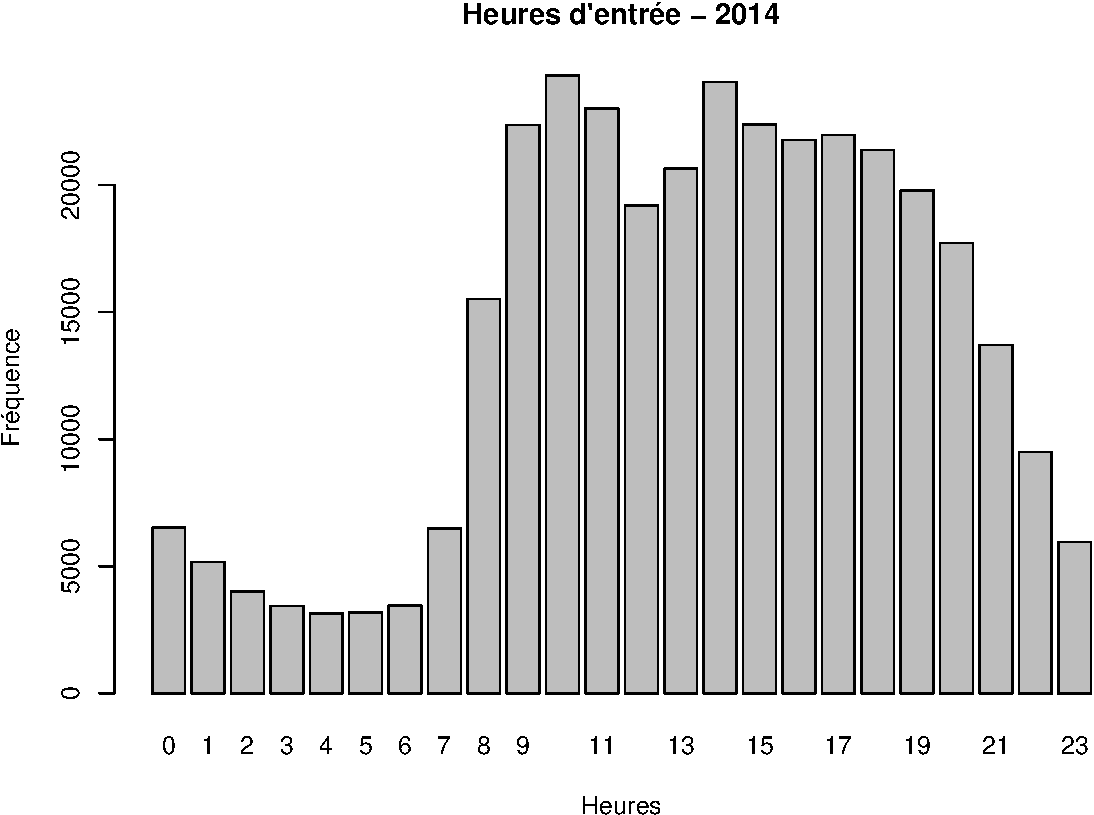
\includegraphics{rapport2014_V4_files/figure-latex/horaires-1.pdf}

\begin{itemize}
\item
  Passages de nuit (20h - 8h): \textbf{24.74 \%} (N = 92 610)
\item
  Passages en nuit profonde (0h - 8h): \textbf{11.09 \%} (N = 41 500)
\item
  Passages en horaire de PDS (8h - 20h): \textbf{45.22 \%}
  \href{Remarque:\%20ne\%20tient\%20pas\%20compte\%20des\%20jours\%20fériés\%20survenant\%20en\%20semaine}{N
  = 188 454}
\end{itemize}

\subsubsection{Variations saisonnières}\label{variations-saisonnieres}

Variation du nombre de RPU entre les mois d'été (juillet-août) et les
autres mois de l'année: \textbf{-5.82 \%}.

\subsubsection{Moyens d'arrivée}\label{moyens-darrivee}

\begin{itemize}
\itemsep1pt\parskip0pt\parsep0pt
\item
  \%(N) d'arrivée personnel: \textbf{72.16 \%} (N = 208 771)
\item
  \%(N) d'arrivée SMUR: \textbf{0.93 \%} (N = 2 702)
\item
  \%(N) d'arrivée VSAB: \textbf{10.35 \%} (N = 29 954)
\item
  \%(N) d'arrivée Ambulance: \textbf{15.94 \%} (N = 46 112)
\end{itemize}

NB : commentaire possible pour expliquer que la somme des 4 pourcentages
ci dessus ne fait pas 100 \%

\subsubsection{Gravité (CCMU)}\label{gravite-ccmu}

\begin{itemize}
\itemsep1pt\parskip0pt\parsep0pt
\item
  nombre de CCMU renseignés: 339827
\item
  \%(N) CCMU 1: \textbf{15.21\%} (n = 51 682)
\item
  \%(N) CCMU 1 et 2: \textbf{84.45\%} (n = 286 979)
\item
  \%(N) CCMU 4 et 5: \textbf{1.28\%} (n = 4 341)
\end{itemize}

Exhaustivité CCMU :

\begin{itemize}
\itemsep1pt\parskip0pt\parsep0pt
\item
  Nombre de RPU 2014 hors orientation = FUGUE, PSA et REO ayant un
  élément transmis pour la CCMU: \textbf{335889}.
\end{itemize}

\subsubsection{Diadnostic principal}\label{diadnostic-principal}

Remarque: les chiffres sont dans le document
\emph{Codes}regroupement\_ORUMIP\_ =\textgreater{} à rajouter.

\begin{itemize}
\itemsep1pt\parskip0pt\parsep0pt
\item
  \% Médico-chirurgical: \textbf{136 816}
\item
  \% Traumatologique: \textbf{91 907}
\item
  \% Psychiatrique: \textbf{6 185}
\item
  \% Toxicologique: \textbf{4 847}
\item
  \% Autres recours: \textbf{7 441}
\end{itemize}

\subsubsection{Durées de passage}\label{durees-de-passage}

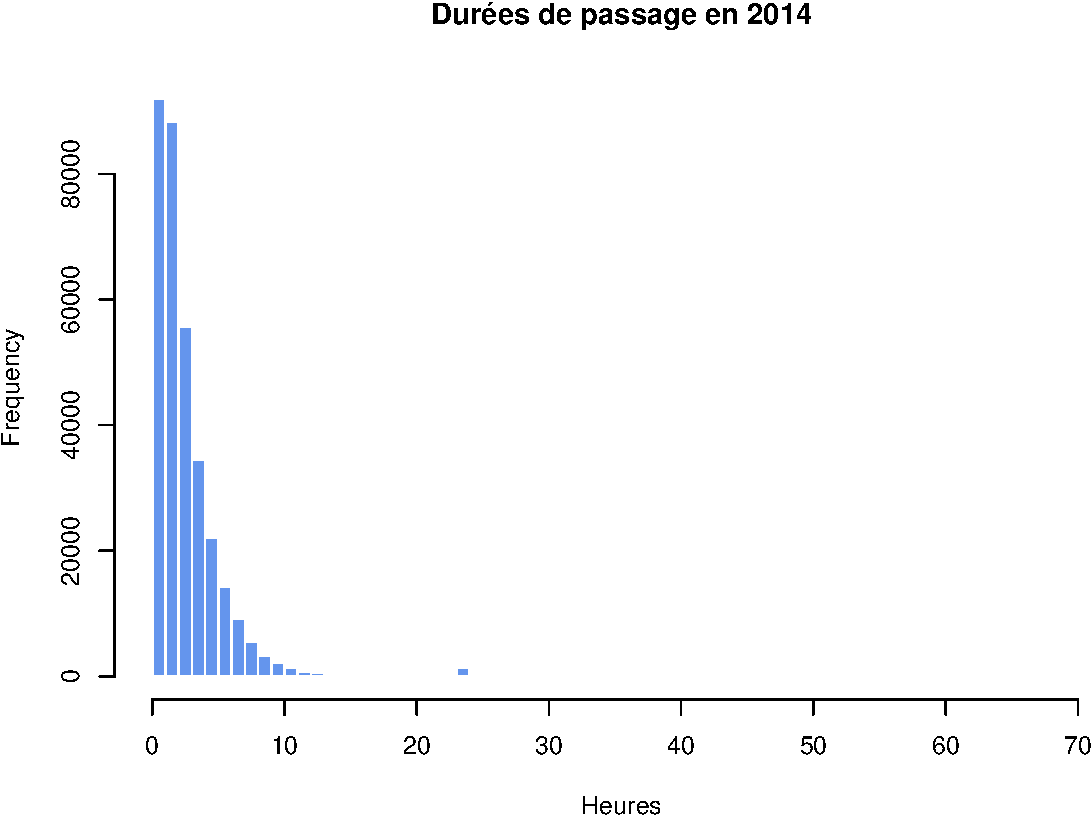
\includegraphics{rapport2014_V4_files/figure-latex/passages-1.pdf}

\begin{itemize}
\item
  Nombre de RPU dont la durée de passage est comprise entre 0h et 72h:
  \textbf{333 397}
\item
  durée moyenne de passage \textbf{156 mn} (2h36).
\item
  écart-type: 176.18 mn (2h56).
\item
  médiane: \textbf{110 mn} (1h50).
\item
  nombre de prises en charge \textgreater{} 4 heures: 62 888
  (\textbf{18.86 \%}).
\item
  nombre de prises en charge inférieures ou égales à 4 heures: 270 509
  (\textbf{81.14 \%}).
\item
  Lors d'une hospitalisation post-urgences (hospitalisation = mutation +
  transfert)

  \begin{itemize}
  \itemsep1pt\parskip0pt\parsep0pt
  \item
    moyenne durée de passage en cas d'hospitalisation: \textbf{187.86
    mn}.
  \item
    médiane durée de passage en cas d'hospitalisation: \textbf{148 mn}.
  \end{itemize}
\item
  Lors d'un retour au domicile

  \begin{itemize}
  \itemsep1pt\parskip0pt\parsep0pt
  \item
    moyenne durée de passage en cas de retour à domicile: \textbf{146.13
    mn}.
  \item
    médiane durée de passage en cas de retour à domicile: \textbf{104
    mn}.
  \end{itemize}
\end{itemize}

(source: temps de passages.Rmd)

\subsubsection{Mode de sortie}\label{mode-de-sortie}

\begin{itemize}
\itemsep1pt\parskip0pt\parsep0pt
\item
  \% (N) de retour à domicile: \textbf{75.5 \%} (N = 255 852)
\item
  \% (N) Hospitalisation: \textbf{24.5 \%} (N = 83 024)
\item
  \% (N) Mutation: \textbf{22.72 \%} (N = 76 999)
\item
  \% (N) Transfert: \textbf{1.78 \%} (N = 6 025)
\item
  Nb de RPU 2014 avec mode de sortie = 6 ou 7 (hospitalisation) avec un
  élément transmis pour la destination: \textbf{82635}
\item
  Nb de RPU 2014 avec mode de sortie = 6 ou 7 avec un élement transmis
  pour l'orientation: \textbf{72898}
\end{itemize}

\section{Les chiffres clés de l'activité des
SAMU}\label{les-chiffres-cles-de-lactivite-des-samu}

(à partir des données SRVA ``officielles'')

\begin{itemize}
\itemsep1pt\parskip0pt\parsep0pt
\item
  Nombre de dossiers de régulation médicale (DRM): 480303
\item
  Nombre de SMUR : 25 321

  \begin{itemize}
  \itemsep1pt\parskip0pt\parsep0pt
  \item
    dont primaires: format.n(19714)
  \end{itemize}
\item
  Nombre d'ambulances privées à la demande du SAMU: format.n(46031)
\end{itemize}

\subsection{Organisation}\label{organisation}

Nombre de colonnes SMUR:

\begin{longtable}[c]{@{}lll@{}}
\toprule\addlinespace
SMUR & Jour & Nuit
\\\addlinespace
\midrule\endhead
Wissembourg & 1 & 1
\\\addlinespace
Haguenau & 1 & 1
\\\addlinespace
Saverne & 1 & 1
\\\addlinespace
Strasbourg & 4 & 3
\\\addlinespace
Sélestat & 1 & 1
\\\addlinespace
Colmar & 2 & 2
\\\addlinespace
Mulhouse & 2 & 2
\\\addlinespace
\bottomrule
\end{longtable}

\section{Les chiffres clés de l'activité pédiatrique des services
d'urgences (moins de 18
ans)}\label{les-chiffres-cles-de-lactivite-pediatrique-des-services-durgences-moins-de-18-ans}

\begin{verbatim}
## ped
##      <28j  28j-1an[   1-5ans[  5-10ans[ 10-15ans[ 15-18ans[ 
##      1791     13554     36287     24738     27012     15800
\end{verbatim}

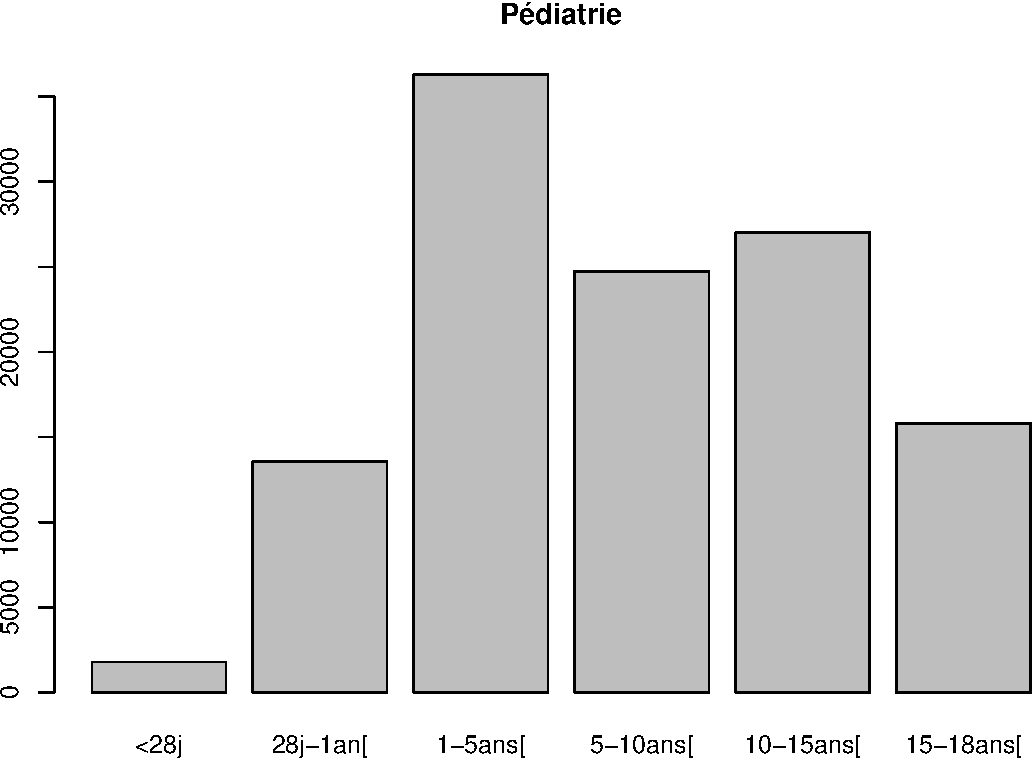
\includegraphics{rapport2014_V4_files/figure-latex/pop18-1.pdf}

\subsection{RECUEIL DES DONNÉES}\label{recueil-des-donnees-1}

\begin{itemize}
\itemsep1pt\parskip0pt\parsep0pt
\item
  Nombre de passages dans l'année: 119 213
\item
  Moyenne quotidienne de passage: 327 passages/j
\item
  Taux d'urgences pédiatriques {[}(Nb RPU Pédia/ Nb RPU global)x100{]}:
  29 \%
\item
  TODO: \% d'évolution par rapport à l'année N-1(données SAE pour ceux
  qui n'ont pas d'historique RPU fiable et permettant la comparaison,
  préciser l'origine des données)
\end{itemize}

\subsection{PATIENTS}\label{patients-1}

\begin{verbatim}
 AMBU    FO  HELI PERSO  SMUR  VSAB        NA's 
 2024    81    17 71809   706  3053     0 41523 
\end{verbatim}

\begin{verbatim}
[1] 77690
\end{verbatim}

\begin{verbatim}
[1] 94706
\end{verbatim}

\begin{verbatim}
    1     2     3     4     5     D     P        NA's 
24353 63361  6678   211    23     2    78     0 24507 
\end{verbatim}

\begin{itemize}
\itemsep1pt\parskip0pt\parsep0pt
\item
  nombre de garçons: 65619
\item
  nombre de filles: 53590
\item
  Sex ratio: 1.22
\item
  Pyramide des âges (âge par année, borne supérieure toujours exclue)
\item
  Par sous classes d'âge:
\end{itemize}

\subsubsection{horaires de passages
pédiatriques}\label{horaires-de-passages-pediatriques}

\begin{itemize}
\itemsep1pt\parskip0pt\parsep0pt
\item
  nombre de passages la nuit: 32677 (p = 27.41 \%)
\item
  nombre de passages en nuit profonde: 8660 (p = 7.26 \%)
\end{itemize}

\subsubsection{Durée de passage}\label{duree-de-passage}

\begin{itemize}
\item
  Nombre de RPU avec une heure de sortie conforme ({]}0-72h{[}: 95936
\item
  Durée moyenne de passage (en min): 121.3 mn
\item
  Durée médiane de passage (en min): 86 mn
\item
  Nombre de RPU dont la durée de passage est inférieure à 4h: 89071
\item
  Nombre de RPU avec une heure de sortie conforme ({]}0-72h{[} lors
  d'une hospitalisation post-urgences: 12452
\item
  Nombre de RPU avec une heure de sortie conforme ({]}0-72h{[} lors d'un
  retour au domicile: 83483
\item
  Nombre de RPU dont la durée de passage est inférieure à 4h lors d'une
  hospitalisation post-urgences: 11313
\item
  Nombre de RPU dont la durée de passage est inférieure à 4h lors d'un
  retour au domicile: 77757
\item
  Nombre de RPU avec un mode de sortie renseigné: 96860
\item
  Nombre de mutation interne: 11996
\item
  Nombre de transfert externe: 556
\item
  nombre de retours à domicile: 84307
\end{itemize}

\section{Les chiffres clés de l'activité gériatrique des services
d'urgences (75 ans et
plus)}\label{les-chiffres-cles-de-lactivite-geriatrique-des-services-durgences-75-ans-et-plus}

\subsection{RECUEIL DES DONNÉES}\label{recueil-des-donnees-2}

\begin{itemize}
\itemsep1pt\parskip0pt\parsep0pt
\item
  Nombre de passages dans l'année: 57 271
\item
  Moyenne quotidienne de passage: 157 passages/j
\item
  Taux d'urgences gériatriques {[}(Nb RPU Géria/ Nb RPU global)x100{]}:
  13.74 \%
\item
  TODO: \% d'évolution par rapport à l'année N-1(données SAE pour ceux
  qui n'ont pas d'historique RPU fiable et permettant la comparaison,
  préciser l'origine des données)
\end{itemize}

\subsection{PATIENTS}\label{patients-2}

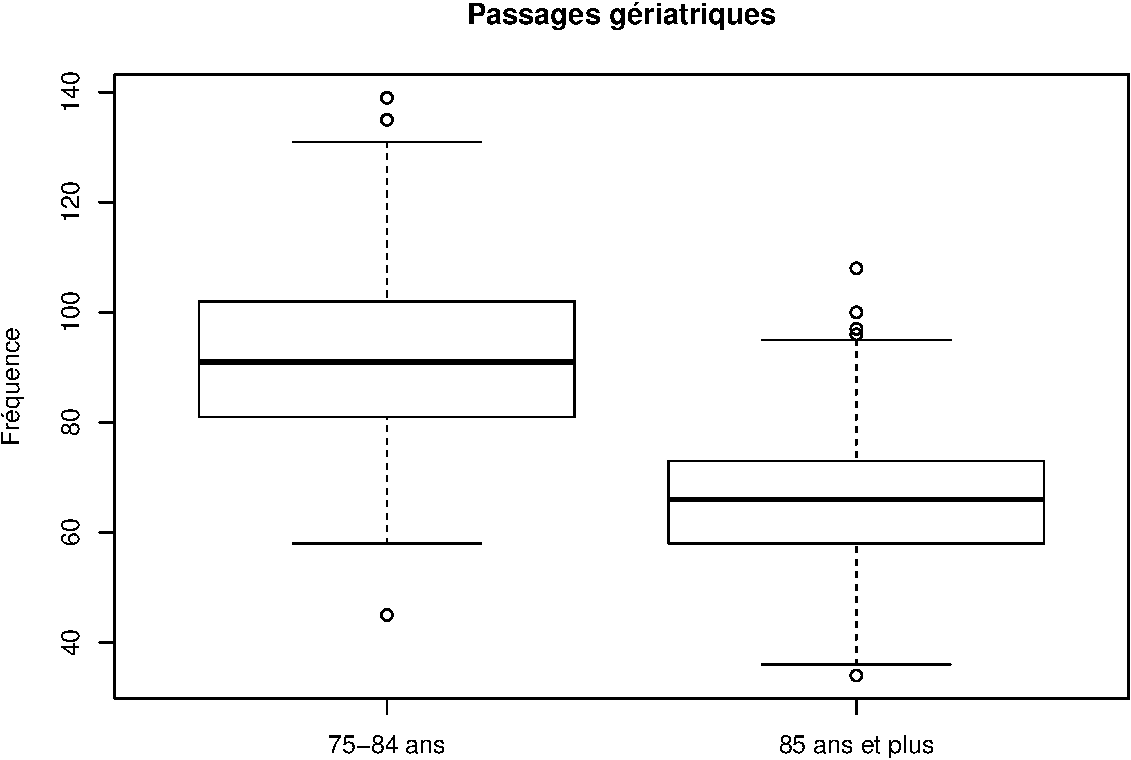
\includegraphics{rapport2014_V4_files/figure-latex/sexe75-1.pdf}

\begin{verbatim}
               effectif moyenne par jour  médiane par jour sex ratio
75-84 ans         33399                92               91      0.82
85 ans et plus    23872                65               66      0.47
\end{verbatim}

\begin{itemize}
\item
  Nombre d'hommes: 22 665
\item
  Nombre de femmes: 34 605
\item
  Sex ratio: 0.65
\item
  Pyramide des âges (âge par année, borne supérieure toujours exclue)
\item
  Par sous classes d'âge:

  \begin{longtable}[c]{@{}rlllc@{}}
  \toprule\addlinespace
  eff & ectif moy & enne par jour méd & iane par jour sex & ratio
  \\\addlinespace
  \midrule\endhead
  75-84 ans & 33399 & 92 & 91 & 0.82
  \\\addlinespace
  85 ans et plus & 23872 & 65 & 66 & 0.47
  \\\addlinespace
  \bottomrule
  \end{longtable}
\end{itemize}

\subsection{ARRIVÉE}\label{arrivee-1}

\subsubsection{Horaires de passage}\label{horaires-de-passage-1}

\begin{itemize}
\itemsep1pt\parskip0pt\parsep0pt
\item
  Nb de RPU avec date/heure d'entrée renseignés: 57 271
\item
  \% passages la nuit: 22.38 \% (N = 12 815)
\item
  \% passages en horaire de PDS: 36.77 \% (N = 21 058)
\end{itemize}

\subsubsection{Moyens de transport}\label{moyens-de-transport}

\begin{itemize}
\item
  nombre de moyens de transport: 57271
\item
  nombre de moyens de transport renseignés: 40878
\item
  nombre de moyens personnels: 11962
\item
  nombre de SMUR: 698
\item
  nombre de VSAV: 6797
\item
  nombre d'ambulances privées: 21370
\item
  \% d'arrivées Moyen perso: 20.89 \% (N = 11 962)
\item
  \% d'arrivées SMUR: 1.22 \% (N = 698)
\item
  \% d'arrivées VSAV: 11.87 \% (N = 6 797)
\item
  \% d'arrivées ambulance privée: 37.31 \% (N = 21 370)
\item
  \% réponses manquantes:
\end{itemize}

NB : commentaire possible pour expliquer que la somme des 4 pourcentages
ci dessus ne fait pas 100 \%

\subsubsection{Gravité}\label{gravite}

\begin{itemize}
\itemsep1pt\parskip0pt\parsep0pt
\item
  Nombre de RPU avec une CCMU renseignée: 47408
\item
  \% CCMU 1: 4.32 \% (N = 2 472)
\item
  \% CCMU 4 et 5: 3.14 \% (N = 1 797)
\end{itemize}

\subsubsection{Diagnostic principal}\label{diagnostic-principal}

\begin{itemize}
\itemsep1pt\parskip0pt\parsep0pt
\item
  \% Médico-chirurgical, dont :

  \begin{itemize}
  \itemsep1pt\parskip0pt\parsep0pt
  \item
    \% cardio vasculaire
  \item
    \% neuro
  \item
    \% digestif
  \item
    \% respiratoire
  \end{itemize}
\item
  \% Traumatologique
\item
  \% Psychiatrique
\item
  \% Toxicologique
\item
  \% Autres recours
\end{itemize}

\subsubsection{DURÉE}\label{duree}

\begin{verbatim}
##        NA  Mutation Transfert  Domicile     Décès           
##        NA       219       316       215        NA        NA
\end{verbatim}

\begin{verbatim}
##        NA  Mutation Transfert  Domicile     Décès           
##        NA       200       248       174        NA        NA
\end{verbatim}

\begin{verbatim}
## 
##  Welch Two Sample t-test
## 
## data:  passages75$duree by passages75$DEVENIR
## t = -4.8, df = 41184, p-value = 0.000001585
## alternative hypothesis: true difference in means is not equal to 0
## 95 percent confidence interval:
##  -12.7  -5.3
## sample estimates:
## mean in group Domicile     mean in group Hosp 
##                    215                    224
\end{verbatim}

\begin{verbatim}
## [1] 0.0000016
\end{verbatim}

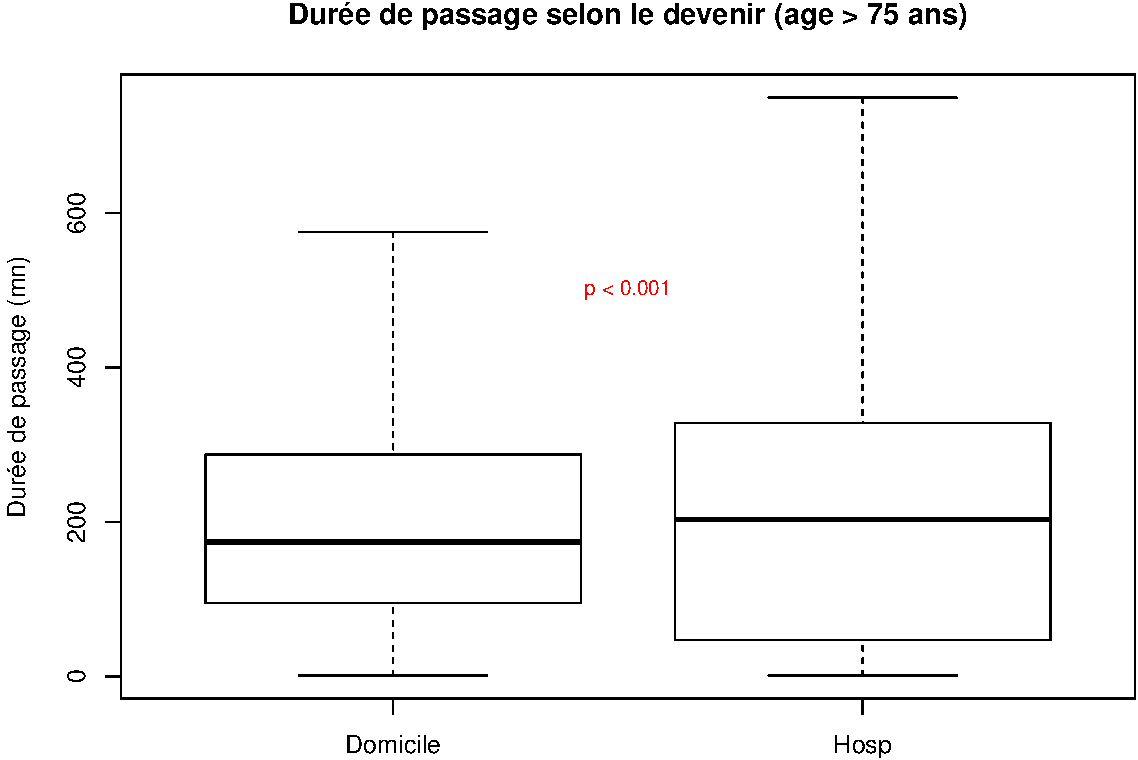
\includegraphics{rapport2014_V4_files/figure-latex/duree_passage_75-1.pdf}

\begin{itemize}
\itemsep1pt\parskip0pt\parsep0pt
\item
  Durée moyenne de passage (HORS UHCD) : 220 minutes
\item
  Durée médiane de passage (HORS UHCD) : 190 minutes
\item
  \% de passages de moins de 4h : 61.22 \%
\item
  lors d'une hospitalisation post-urgences (hospitalisation = mutation +
  transfert): 223.7 minutes.
\item
  lors d'un retour au domicile: 214.71 minutes.
\end{itemize}

\paragraph{Nouveau}\label{nouveau}

\begin{itemize}
\item
  Nombre de RPU avec une heure de sortie conforme ({]}0-72h{[}: 45715
\item
  Durée moyenne de passage (en min): 220.66 mn
\item
  Durée médiane de passage (en min): 190 mn
\item
  Nombre de RPU dont la durée de passage est inférieure à 4h: 27982
\item
  Nombre de RPU avec une heure de sortie conforme ({]}0-72h{[} lors
  d'une hospitalisation post-urgences: 28228
\item
  Nombre de RPU avec une heure de sortie conforme ({]}0-72h{[} lors d'un
  retour au domicile: 17487
\item
  Nombre de RPU dont la durée de passage est inférieure à 4h lors d'une
  hospitalisation post-urgences: 16467
\item
  Nombre de RPU dont la durée de passage est inférieure à 4h lors d'un
  retour au domicile: 11515
\end{itemize}

\subsubsection{MODE DE SORTIE}\label{mode-de-sortie-1}

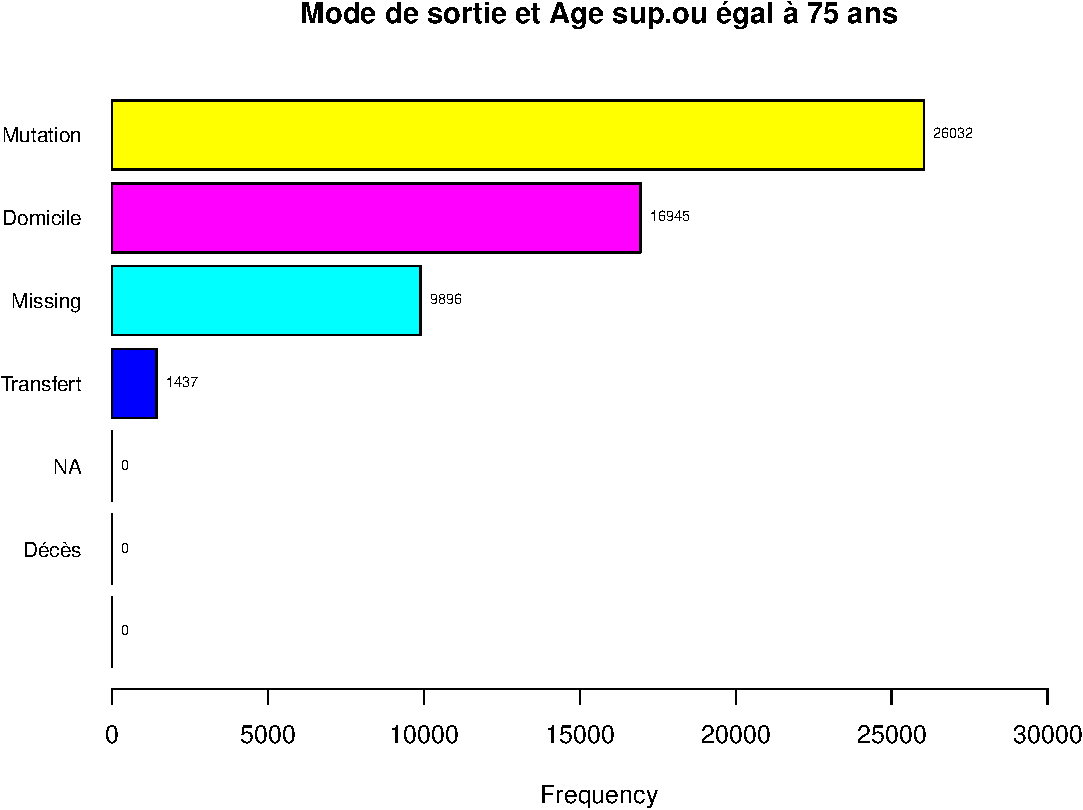
\includegraphics{rapport2014_V4_files/figure-latex/sortie75-1.pdf}

\begin{verbatim}
## pop75$MODE_SORTIE : 
##           Frequency   %(NA+)   %(NA-)
## Mutation      27196     47.5     58.1
## Domicile      18131     31.7     38.7
## NA's          10430     18.2      0.0
## Transfert      1514      2.6      3.2
## NA                0      0.0      0.0
## Décès             0      0.0      0.0
##                   0      0.0      0.0
##   Total       57271    100.0    100.0
\end{verbatim}

\begin{itemize}
\itemsep1pt\parskip0pt\parsep0pt
\item
  \% d'hospitalisation: 50.13 \% (N = 28 710)

  \begin{itemize}
  \itemsep1pt\parskip0pt\parsep0pt
  \item
    \% de mutation:47.49 \% (N = 27 196)
  \item
    \% de transfert:2.64 \% (N = 1 514)
  \end{itemize}
\item
  \% de retour à domicile:31.66 \% (N = 18 131)
\end{itemize}

\paragraph{rapport régional}\label{rapport-regional}

\begin{itemize}
\itemsep1pt\parskip0pt\parsep0pt
\item
  Nombre de RPU avec un mode de sortie renseigné: 46 841
\item
  Nombre de mutation interne: 27 196
\item
  Nombre de transfert externe: 1 514
\item
  nombre de retours à domicile: 18 131
\end{itemize}

\section{Les chiffres clés de l'activité AVC des services
d'urgences}\label{les-chiffres-cles-de-lactivite-avc-des-services-durgences}

\subsection{RECUEIL DES DONNÉES}\label{recueil-des-donnees-3}

\begin{itemize}
\itemsep1pt\parskip0pt\parsep0pt
\item
  Nombre d'AVC dans l'année (+ rappeler le pourcentage d'exhaustivité du
  DP par rapport au nombre de RPU): \textbf{2 949}
\item
  Moyenne quotidienne d'AVC: \textbf{8,1 AVC/j}
\item
  \% d'AVC dans l'activité globale: \textbf{1.19 \%}
\end{itemize}

\subsection{Répartition des AVC}\label{repartition-des-avc}

Exemple d'utilisation de la méthode \emph{hist} appliquée aux objets
date-time:

\begin{itemize}
\itemsep1pt\parskip0pt\parsep0pt
\item
  \emph{x} = as.Date(AVC\$ENTREE)
\item
  \emph{breaks} est obligatoire: ``days'', ``weeks'', ``months'',
  ``quarters'', ``years'', ``secs'', ``mins'', ``hours''. Utiliser
  \emph{start.on.monday = TRUE} si \emph{breaks = ``weeks''}.
\item
  \emph{freq} = TRUE (défaut FALSE) pour afficher les fréquences
\item
  \emph{format} permet de coisir l'affichage de la date sur l'axe des x
  \href{https://stat.ethz.ch/R-manual/R-devel/library/base/html/strptime.html}{voir}.
\end{itemize}

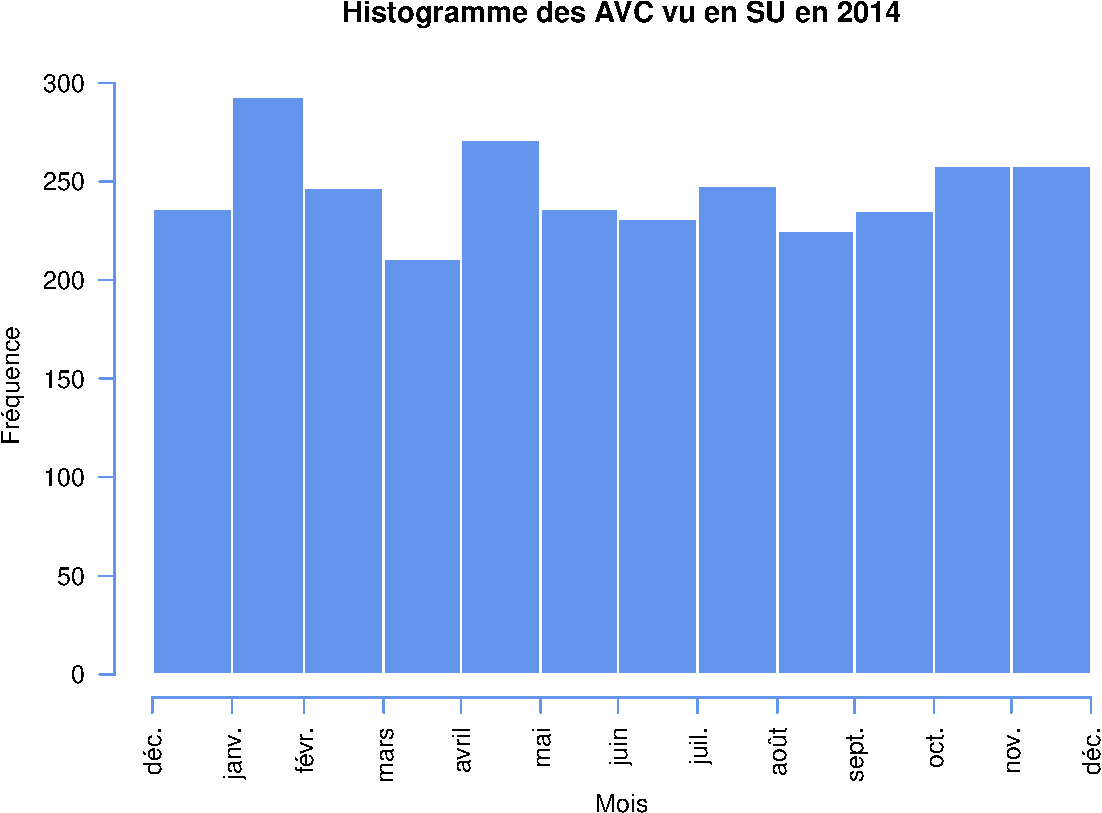
\includegraphics{rapport2014_V4_files/figure-latex/hist_avc-1.pdf}

\subsection{PATIENTS}\label{patients-3}

\begin{verbatim}
## c.age
##     [0,5)    [5,10)   [10,15)   [15,20)   [20,25)   [25,30)   [30,35) 
##        10         2         4        10        19        26        26 
##   [35,40)   [40,45)   [45,50)   [50,55)   [55,60)   [60,65)   [65,70) 
##        33        68        97       150       166       235       284 
##   [70,75)   [75,80)   [80,85)   [85,90)   [90,95)  [95,100) [100,105) 
##       295       393       496       408       193        28         4 
## [105,110) [110,115) [115,120) 
##         1         1         0
\end{verbatim}

\includegraphics{rapport2014_V4_files/figure-latex/patients-1.pdf}

\begin{verbatim}
## c.age
##    [0,1)    [1,5)   [5,10)  [10,15)  [15,18)  [18,30)  [30,45)  [45,65) 
##        3        7        2        4        4       51      127      648 
##  [65,75)  [75,85) [85,120) 
##      579      889      635
\end{verbatim}

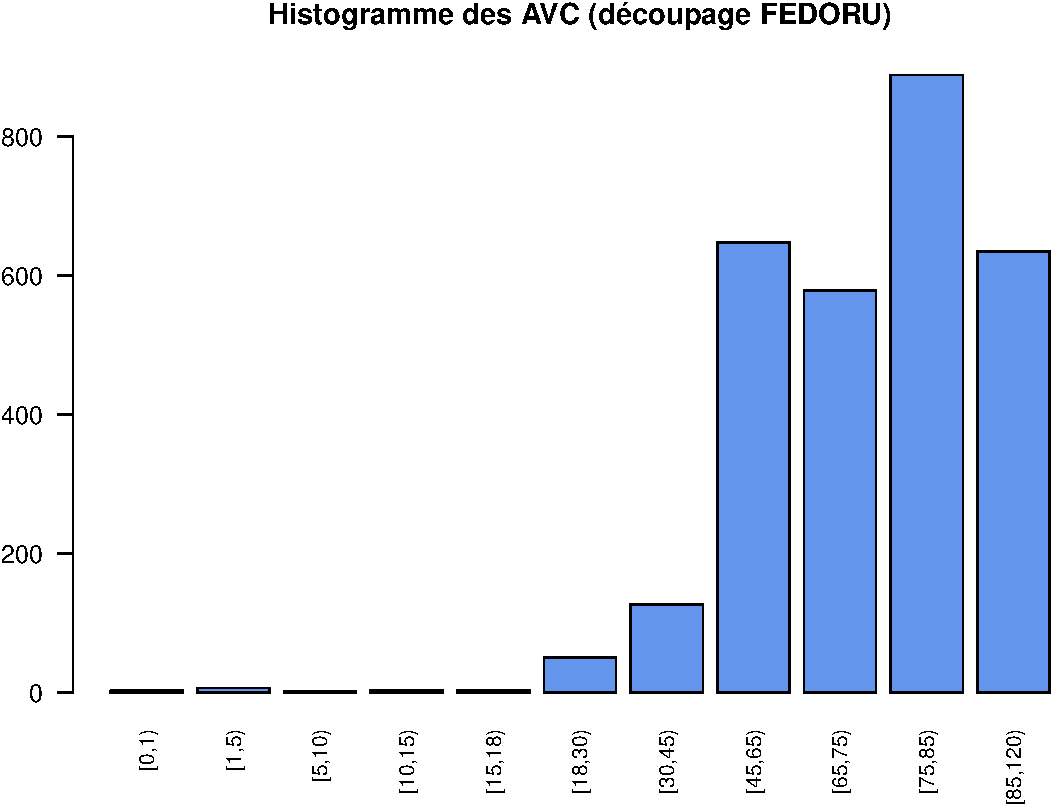
\includegraphics{rapport2014_V4_files/figure-latex/patients-2.pdf}

\begin{itemize}
\itemsep1pt\parskip0pt\parsep0pt
\item
  Sex ratio: 0.95
\item
  Age moyen: 71.44 ans
\item
  Nombre d'AVC par sous classe d'âge (GT1):
\end{itemize}

\subsection{ARRIVÉE}\label{arrivee-2}

\begin{itemize}
\itemsep1pt\parskip0pt\parsep0pt
\item
  Nombre d'AVC et \% par tranche d'heure GT1 (matinée, début d'après
  midi, fin d'après midi, soirée, nuit profonde)
\end{itemize}

\begin{verbatim}
##      nuit profonde matinée  début après-midi fin après-midi soirée   
## [1,] "[0,8)"       "[8,12)" "[12,16)"        "[16,20)"      "[20,24)"
## [2,] "272"         "900"    "865"            "619"          "293"
\end{verbatim}

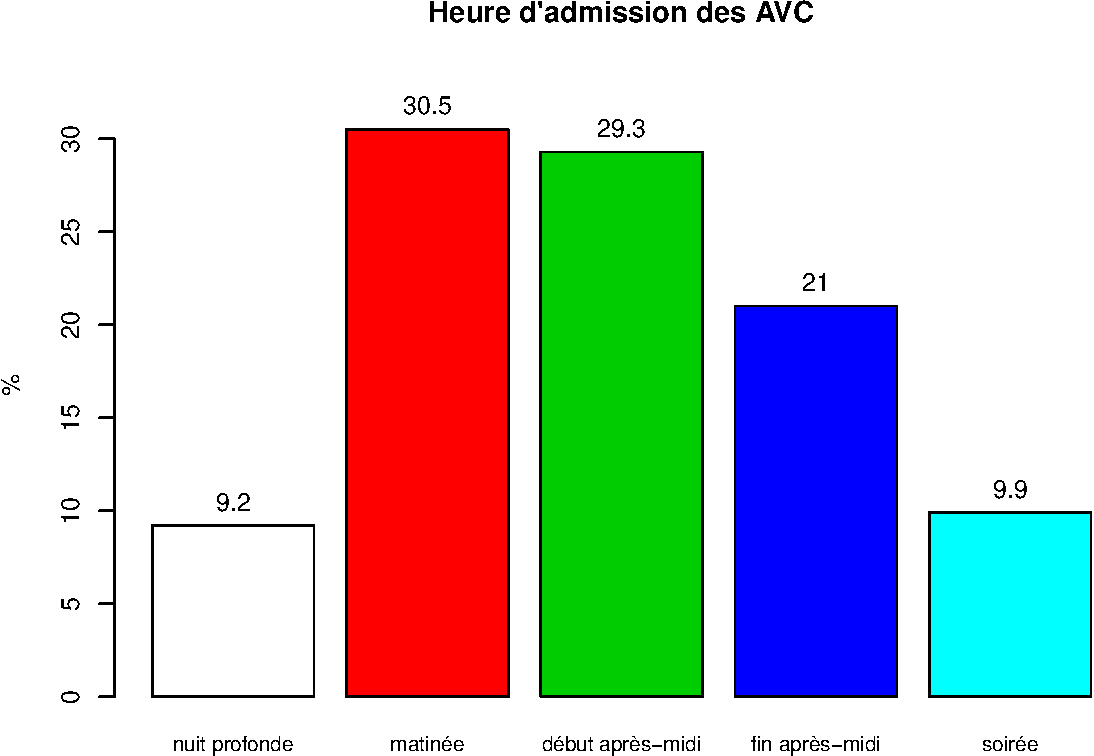
\includegraphics{rapport2014_V4_files/figure-latex/avc_periode-1.pdf}

\begin{itemize}
\item
  \% AVC le matin: 30.5 \%.
\item
  \% AVC en début d'après-midi: 29.3 \%.
\item
  \% AVC en fin d'après-midi: 21 \%.
\item
  \% AVC en soirée: 9.9 \%.
\item
  \% AVC le nuit profonde: 9.2 \%.
\item
  Nombre de passages AVC urgences, déclinaison par département,
  établissement, année N
\end{itemize}

\begin{verbatim}
## 3Fr Alk Ane Col Dia Dts Geb Hag Hus Mul Odi Ros Sav Sel Wis 
##  63  30  NA 741  NA  NA  30 500 580 682  NA  NA  NA 238  85
\end{verbatim}

\begin{itemize}
\item
  \% passages en horaire de PDS

  \begin{longtable}[c]{@{}rlll@{}}
  \toprule\addlinespace
  PDS & S PDS & WE NPD & S
  \\\addlinespace
  \midrule\endhead
  Nombre AVC & 403 & 656 & 1890
  \\\addlinespace
  \% AVC & 14 & 22 & 64
  \\\addlinespace
  \bottomrule
  \end{longtable}
\end{itemize}

PDSS = horaires de PDS en semaine, PDSWE = horaires de PDS le WE, NPDS =
hors horaire de PDS.

\begin{itemize}
\itemsep1pt\parskip0pt\parsep0pt
\item
  nombre d'AVC aux horaires de PDS en semaine: 13.67 \%
\item
  nombre d'AVC aux horaires de PDS de week-end:22.24 \%
\item
  nombre d'AVC en dehors des horaires de PDS:64.09 \%
\item
  Nombre de RPU avec diag AVC avec date et heure d'entrées renseignées:
  2 949
\end{itemize}

\subsection{Mode d'arrivée aux
urgences}\label{mode-darrivee-aux-urgences}

\begin{verbatim}
##       n    n.na    p.na  n.rens  p.rens      FO    HELI   PERSO    SMUR 
## 2949.00  554.00    0.19 2395.00    0.81    1.00   19.00  636.00   58.00 
##    VSAB    AMBU 
##  527.00 1154.00
\end{verbatim}

\begin{itemize}
\itemsep1pt\parskip0pt\parsep0pt
\item
  Nombre de RPU avec moyens de transport précisé: 2 395
\item
  \% d'arrivées Moyen perso: 21.57\%
\item
  \% d'arrivées SMUR: 1.97\%
\item
  \% d'arrivées VSAV: NA\%
\item
  \% d'arrivées ambulance privée: 39.13\% NB : commentaire possible pour
  expliquer que la somme des 4 pourcentages ci dessus ne fait pas 100 \%
\end{itemize}

\subsection{Diagnostic principal}\label{diagnostic-principal-1}

\begin{itemize}
\itemsep1pt\parskip0pt\parsep0pt
\item
  Nombre d'AVC ischémiques et \%: 1 021 (34.62 \%)
\item
  Nombre d'AVC hémorragiques et \%: 442 (14.99 \%)
\item
  Nombre d'AIT et \%: 806 (27.33 \%)
\item
  Nombre de codes ``symptomatiques'' (hémiplégie, aphasie, amaurose,
  etc\ldots{}) et \%: 680 (23.06 \%)
\end{itemize}

NB : se référer à l'annexe 4 pour les regroupements.

\subsection{DURÉE}\label{duree-1}

Voir ligne 333

Voir les routines de RPU\_2014/Analyse/Temps\_passage/passage.R et
notamment \textbf{temps de passage}.

\begin{itemize}
\item
  Nombre de RPU avec une heure de sortie conforme ({]}0-72h{[}: 2 564
\item
  Durée moyenne de passage des patients PEC pour AVC (en min): 250
\item
  Durée médiane de passage des patients PEC pour AVC (en min): 229
\item
  Nombre de RPU ac diag AVC dont la durée de passage est inférieure à
  4h: 1 352
\item
  Durée de passage (HORS UHCD) année N: moyenne \textbf{249.8} minutes,
  et médiane \textbf{228} minutes.
\item
  \% de passages de moins de 4h 0.92
\end{itemize}

\subsection{MODE DE SORTIE}\label{mode-de-sortie-2}

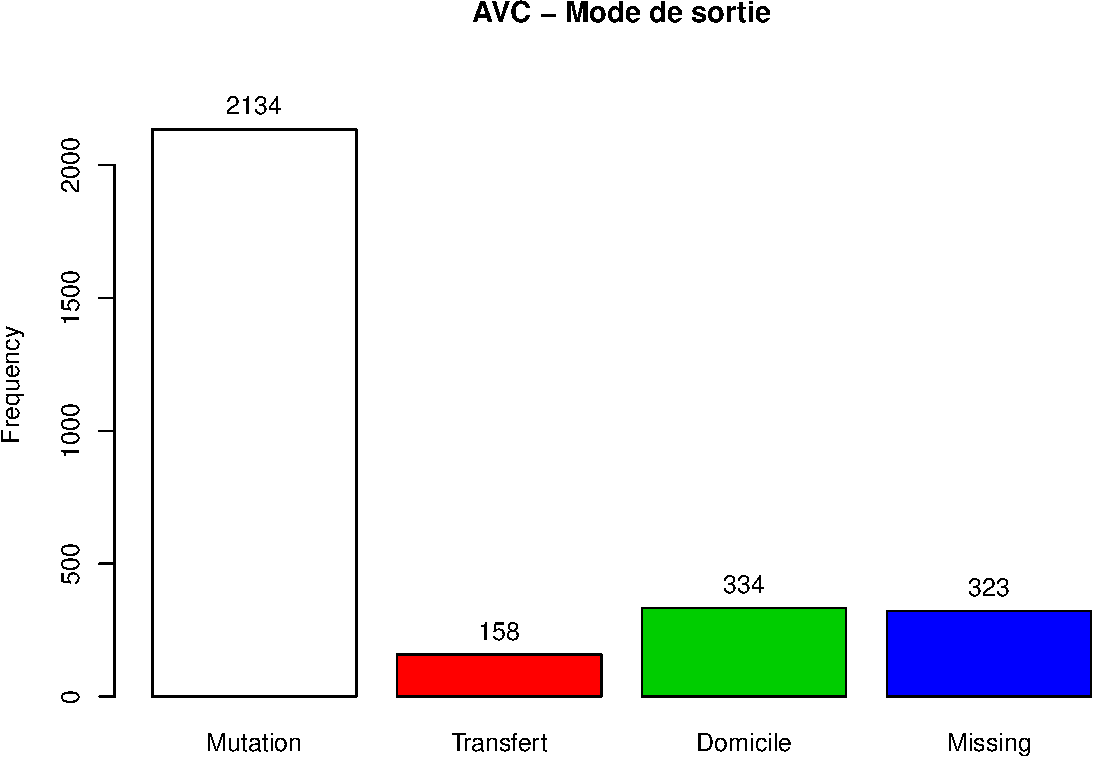
\includegraphics{rapport2014_V4_files/figure-latex/avc_mode_sortie-1.pdf}

\begin{itemize}
\itemsep1pt\parskip0pt\parsep0pt
\item
  Nombre de RPU ac diag. AVC avec un mode de sortie renseigné: 2626
\item
  \% d'hospitalisation: 87.3 \% (N = 2292)
\item
  \% de mutation: 81.3 \% (N = 2134)
\item
  \% de transfert: 6 \% (N = 158)
\item
  \% de retour à domicile: 12.7 \% (N = 334)
\end{itemize}

\subsection{Orientation}\label{orientation}

\begin{itemize}
\itemsep1pt\parskip0pt\parsep0pt
\item
  Répartition par orientation en pourcentage, année N
\end{itemize}

\% Table created by stargazer v.5.2 by Marek Hlavac, Harvard University.
E-mail: hlavac at fas.harvard.edu \% Date and time: Jeu, aoû 20, 2015 -
19:13:54

\begin{table}[!htbp] \centering 
  \caption{Orientation des AVC} 
  \label{orientation} 
\begin{tabular}{@{\extracolsep{5pt}} cccccccccc} 
\\[-1.8ex]\hline 
\hline \\[-1.8ex] 
CHIR & FUGUE & HO & MED & REA & SC & SCAM & SI & UHCD & NA's \\ 
\hline \\[-1.8ex] 
$75$ & $1$ & $1$ & $720$ & $68$ & $46$ & $9$ & $361$ & $919$ & $749$ \\ 
\hline \\[-1.8ex] 
\end{tabular} 
\end{table}

\section{Analyse par type
d'étblissement}\label{analyse-par-type-detblissement}

Voir routine \textbf{analyse-type\_etablissement} (rapport\_2014.R).

\subsection{SU de CHU}\label{su-de-chu}

Un seul établissement \textbf{HUS} avec 3 SU:

\begin{itemize}
\itemsep1pt\parskip0pt\parsep0pt
\item
  NHC
\item
  HTP Adultes
\item
  HTP Pédiatrie
\end{itemize}

\begin{verbatim}
## [1] 61793
\end{verbatim}

\begin{verbatim}
##          n       n.na       p.na     n.rens     p.rens   n.inf1an 
##  61793.000      0.000      0.000  61793.000      1.000  15376.000 
## n.inf15ans n.inf18ans    n.75ans    n.85ans    n.90ans   p.inf1an 
## 103413.000 119213.000  57271.000  23872.000   9487.000      0.037 
## p.inf15ans p.inf18ans    p.75ans    p.85ans    p.90ans   mean.age 
##      0.248      0.286      0.137      0.057      0.023     42.400 
##     sd.age median.age    min.age    max.age         q1         q3 
##     29.320     41.000      0.000    110.000     16.000     68.000
\end{verbatim}

\begin{verbatim}
##           n        n.na        p.na      n.rens      p.rens n.residents 
##       61793           0           0       61793           1       59288 
## n.etrangers 
##        2505
\end{verbatim}

\begin{verbatim}
##  Lun  Mar  Mer  Jeu  Ven  Sam  Dim 
## 9211 8980 8527 8667 9170 8806 8432
\end{verbatim}

\begin{verbatim}
##          n       n.na       p.na     n.rens     p.rens   n.inf1an 
##  61793.000      0.000      0.000  61793.000      1.000  15376.000 
## n.inf15ans n.inf18ans    n.75ans    n.85ans    n.90ans   p.inf1an 
## 103413.000 119213.000  57271.000  23872.000   9487.000      0.037 
## p.inf15ans p.inf18ans    p.75ans    p.85ans    p.90ans   mean.age 
##      0.248      0.286      0.137      0.057      0.023     42.400 
##     sd.age median.age    min.age    max.age         q1         q3 
##     29.320     41.000      0.000    110.000     16.000     68.000
\end{verbatim}

\begin{verbatim}
## [1] 22681.00     0.37
\end{verbatim}

\begin{verbatim}
## 
##  NPDS  PDSS PDSWE 
## 31429 14830 15534
\end{verbatim}

\begin{verbatim}
##      n   n.na   p.na n.rens p.rens 
##  61793      0      0  61793      1
\end{verbatim}

\begin{verbatim}
##        n     n.na     p.na   n.rens   p.rens       FO     HELI    PERSO 
## 61793.00 53476.00     0.87  8317.00     0.13    47.00     2.00  1214.00 
##     SMUR     VSAB     AMBU 
##   274.00  2262.00  4518.00
\end{verbatim}

\begin{verbatim}
##        n     n.na     p.na   n.rens   p.rens    CCMU1    CCMU2    CCMU3 
## 61793.00 28298.00     0.46 33495.00     0.54  8743.00 17870.00  6178.00 
##    CCMU4    CCMU5   CCMU P   CCMU D 
##   503.00   201.00       NA       NA
\end{verbatim}

\begin{verbatim}
##                 n.conforme      duree.moyenne.passage 
##                      26292                        159 
##      duree.mediane.passage  duree.moyenne.passage.dom 
##                          1                        827 
##  duree.mediane.passage.dom duree.moyenne.passage.hosp 
##                        663                         75 
## duree.mediane.passage.hosp                 n.passage4 
##                          1                      20805 
##            n.hosp.passage4             n.dom.passage4 
##                      20137                        668 
##                      n.dom                     n.hosp 
##                       2959                      23333 
##                n.transfert                 n.mutation 
##                        115                      23218 
##                    n.deces 
##                          0
\end{verbatim}

\begin{verbatim}
##           n        n.na        p.na      n.rens      p.rens       n.dom 
##    61793.00    35337.00        0.57    26456.00        0.43     3122.00 
##      n.hosp n.transfert  n.mutation     n.deces 
##    23334.00      115.00    23219.00        0.00
\end{verbatim}

\subsection{SU d'ES siège de SAMU, non
CHU}\label{su-des-siege-de-samu-non-chu}

Un seul établissement: CH de Mulhouse avec 2 implantations:

\begin{itemize}
\itemsep1pt\parskip0pt\parsep0pt
\item
  Emile Muller (Adultes + Pédiatrie traumatique)
\item
  Hasenrain (Pédiatrie médicale)
\end{itemize}

\begin{verbatim}
[1] 59471
\end{verbatim}

\begin{verbatim}
         n       n.na       p.na     n.rens     p.rens   n.inf1an 
 59471.000      0.000      0.000  59471.000      1.000  15376.000 
n.inf15ans n.inf18ans    n.75ans    n.85ans    n.90ans   p.inf1an 
103413.000 119213.000  57271.000  23872.000   9487.000      0.037 
p.inf15ans p.inf18ans    p.75ans    p.85ans    p.90ans   mean.age 
     0.248      0.286      0.137      0.057      0.023     34.600 
    sd.age median.age    min.age    max.age         q1         q3 
    28.078     30.000      0.000    113.000      8.000     57.000 
\end{verbatim}

\begin{verbatim}
          n        n.na        p.na      n.rens      p.rens n.residents 
      59471           0           0       59471           1       57952 
n.etrangers 
       1519 
\end{verbatim}

\begin{verbatim}
 Lun  Mar  Mer  Jeu  Ven  Sam  Dim 
8868 7885 8130 7931 8270 8854 9533 
\end{verbatim}

\begin{verbatim}
         n       n.na       p.na     n.rens     p.rens   n.inf1an 
 59471.000      0.000      0.000  59471.000      1.000  15376.000 
n.inf15ans n.inf18ans    n.75ans    n.85ans    n.90ans   p.inf1an 
103413.000 119213.000  57271.000  23872.000   9487.000      0.037 
p.inf15ans p.inf18ans    p.75ans    p.85ans    p.90ans   mean.age 
     0.248      0.286      0.137      0.057      0.023     34.600 
    sd.age median.age    min.age    max.age         q1         q3 
    28.078     30.000      0.000    113.000      8.000     57.000 
\end{verbatim}

\begin{verbatim}
[1] 18349.00     0.31
\end{verbatim}

\begin{verbatim}

 NPDS  PDSS PDSWE 
31661 11503 16307 
\end{verbatim}

\begin{verbatim}
     n   n.na   p.na n.rens p.rens 
 59471      0      0  59471      1 
\end{verbatim}

\begin{verbatim}
        n      n.na      p.na    n.rens    p.rens        FO      HELI 
59471.000  3836.000     0.065 55635.000     0.935   478.000   122.000 
    PERSO      SMUR      VSAB      AMBU 
35973.000   223.000  7051.000 11788.000 
\end{verbatim}

\begin{verbatim}
       n     n.na     p.na   n.rens   p.rens    CCMU1    CCMU2    CCMU3 
59471.00 14043.00     0.24 45428.00     0.76  7349.00 30451.00  6094.00 
   CCMU4    CCMU5   CCMU P   CCMU D 
 1235.00   299.00       NA       NA 
\end{verbatim}

\begin{verbatim}
                n.conforme      duree.moyenne.passage 
                     43850                        189 
     duree.mediane.passage  duree.moyenne.passage.dom 
                       153                        175 
 duree.mediane.passage.dom duree.moyenne.passage.hosp 
                       142                        254 
duree.mediane.passage.hosp                 n.passage4 
                       224                      31491 
           n.hosp.passage4             n.dom.passage4 
                      4238                      27253 
                     n.dom                     n.hosp 
                     35953                       7897 
               n.transfert                 n.mutation 
                       146                       7751 
                   n.deces 
                         0 
\end{verbatim}

\begin{verbatim}
          n        n.na        p.na      n.rens      p.rens       n.dom 
   59471.00    14257.00        0.24    45214.00        0.76    36717.00 
     n.hosp n.transfert  n.mutation     n.deces 
    8497.00      150.00     8347.00        0.00 
\end{verbatim}

\subsection{SU avec SMUR non siège de
SAMU}\label{su-avec-smur-non-siege-de-samu}

SU abec SMUR sans SAMU, 5 établissements:

\begin{itemize}
\itemsep1pt\parskip0pt\parsep0pt
\item
  CH Wissembourg
\item
  CH haguenau
\item
  CH Saverne
\item
  CH Sélestat
\item
  CH Colmar
\end{itemize}

\begin{verbatim}
[1] 177747
\end{verbatim}

\begin{verbatim}
         n       n.na       p.na     n.rens     p.rens   n.inf1an 
177747.000      0.000      0.000 177747.000      1.000  15376.000 
n.inf15ans n.inf18ans    n.75ans    n.85ans    n.90ans   p.inf1an 
103413.000 119213.000  57271.000  23872.000   9487.000      0.037 
p.inf15ans p.inf18ans    p.75ans    p.85ans    p.90ans   mean.age 
     0.248      0.286      0.137      0.057      0.023     37.300 
    sd.age median.age    min.age    max.age         q1         q3 
    27.737     33.000      0.000    120.000     13.000     59.000 
\end{verbatim}

\begin{verbatim}
          n        n.na        p.na      n.rens      p.rens n.residents 
     177747           0           0      177747           1      166676 
n.etrangers 
      11071 
\end{verbatim}

\begin{verbatim}
  Lun   Mar   Mer   Jeu   Ven   Sam   Dim 
27415 24007 24628 24099 24688 25896 27014 
\end{verbatim}

\begin{verbatim}
         n       n.na       p.na     n.rens     p.rens   n.inf1an 
177747.000      0.000      0.000 177747.000      1.000  15376.000 
n.inf15ans n.inf18ans    n.75ans    n.85ans    n.90ans   p.inf1an 
103413.000 119213.000  57271.000  23872.000   9487.000      0.037 
p.inf15ans p.inf18ans    p.75ans    p.85ans    p.90ans   mean.age 
     0.248      0.286      0.137      0.057      0.023     37.300 
    sd.age median.age    min.age    max.age         q1         q3 
    27.737     33.000      0.000    120.000     13.000     59.000 
\end{verbatim}

\begin{verbatim}
[1] 46677.00     0.26
\end{verbatim}

\begin{verbatim}

  NPDS   PDSS  PDSWE 
101652  29361  46734 
\end{verbatim}

\begin{verbatim}
     n   n.na   p.na n.rens p.rens 
177747      0      0 177747      1 
\end{verbatim}

\begin{verbatim}
        n      n.na      p.na    n.rens    p.rens        FO      HELI 
177747.00  41213.00      0.23 136534.00      0.77    760.00     95.00 
    PERSO      SMUR      VSAB      AMBU 
 97489.00   1603.00  14816.00  21771.00 
\end{verbatim}

\begin{verbatim}
        n      n.na      p.na    n.rens    p.rens     CCMU1     CCMU2 
177747.00  21649.00      0.12 156098.00      0.88  27108.00 101455.00 
    CCMU3     CCMU4     CCMU5    CCMU P    CCMU D 
 24309.00   1547.00    385.00   1273.00     21.00 
\end{verbatim}

\begin{verbatim}
                n.conforme      duree.moyenne.passage 
                    165658                        168 
     duree.mediane.passage  duree.moyenne.passage.dom 
                       124                        144 
 duree.mediane.passage.dom duree.moyenne.passage.hosp 
                       107                        245 
duree.mediane.passage.hosp                 n.passage4 
                       211                     130119 
           n.hosp.passage4             n.dom.passage4 
                     23133                     106985 
                     n.dom                     n.hosp 
                    125512                      40145 
               n.transfert                 n.mutation 
                      2958                      37187 
                   n.deces 
                         1 
\end{verbatim}

\begin{verbatim}
          n        n.na        p.na      n.rens      p.rens       n.dom 
 177747.000   10215.000       0.057  167532.000       0.943  126977.000 
     n.hosp n.transfert  n.mutation     n.deces 
  40554.000    2990.000   37564.000       1.000 
\end{verbatim}

\subsection{SU non SMUR, non SAMU, non
CHU}\label{su-non-smur-non-samu-non-chu}

ES avec SU isolé (pas de SMUR associé): 8 établissements

\begin{itemize}
\itemsep1pt\parskip0pt\parsep0pt
\item
  Ste Anne
\item
  Ste Odile
\item
  Diaconat Strasbourg
\item
  CH de Guebwiller
\item
  CH de Thann (pas de RPU)
\item
  CH d'Altkirch
\item
  Clinique des 3 frontières
\item
  Roosvelt
\item
  Fonderie
\end{itemize}

\begin{verbatim}
[1] 117722
\end{verbatim}

\begin{verbatim}
            n          n.na          p.na        n.rens        p.rens 
117722.000000      4.000000      0.000034 117718.000000      0.999966 
     n.inf1an    n.inf15ans    n.inf18ans       n.75ans       n.85ans 
 15376.000000 103413.000000 119213.000000  57271.000000  23872.000000 
      n.90ans      p.inf1an    p.inf15ans    p.inf18ans       p.75ans 
  9487.000000      0.036897      0.248154      0.286068      0.137430 
      p.85ans       p.90ans      mean.age        sd.age    median.age 
     0.057284      0.022765     38.500000     23.926814     35.000000 
      min.age       max.age            q1            q3 
     0.000000    108.000000     19.000000     56.000000 
\end{verbatim}

\begin{verbatim}
          n        n.na        p.na      n.rens      p.rens n.residents 
     117722           0           0      117722           1      114350 
n.etrangers 
       3372 
\end{verbatim}

\begin{verbatim}
  Lun   Mar   Mer   Jeu   Ven   Sam   Dim 
18645 15880 16232 16002 16456 17567 16940 
\end{verbatim}

\begin{verbatim}
            n          n.na          p.na        n.rens        p.rens 
117722.000000      4.000000      0.000034 117718.000000      0.999966 
     n.inf1an    n.inf15ans    n.inf18ans       n.75ans       n.85ans 
 15376.000000 103413.000000 119213.000000  57271.000000  23872.000000 
      n.90ans      p.inf1an    p.inf15ans    p.inf18ans       p.75ans 
  9487.000000      0.036897      0.248154      0.286068      0.137430 
      p.85ans       p.90ans      mean.age        sd.age    median.age 
     0.057284      0.022765     38.500000     23.926814     35.000000 
      min.age       max.age            q1            q3 
     0.000000    108.000000     19.000000     56.000000 
\end{verbatim}

\begin{verbatim}
[1] 27711.00     0.24
\end{verbatim}

\begin{verbatim}

 NPDS  PDSS PDSWE 
70145 17768 29809 
\end{verbatim}

\begin{verbatim}
     n   n.na   p.na n.rens p.rens 
117722      0      0 117722      1 
\end{verbatim}

\begin{verbatim}
        n      n.na      p.na    n.rens    p.rens        FO      HELI 
117722.00  28900.00      0.25  88822.00      0.75    264.00      1.00 
    PERSO      SMUR      VSAB      AMBU 
 74095.00    602.00   5825.00   8035.00 
\end{verbatim}

\begin{verbatim}
        n      n.na      p.na    n.rens    p.rens     CCMU1     CCMU2 
117722.00  12916.00      0.11 104806.00      0.89   8482.00  85521.00 
    CCMU3     CCMU4     CCMU5    CCMU P    CCMU D 
 10593.00    147.00     24.00     34.00      5.00 
\end{verbatim}

\begin{verbatim}
                n.conforme      duree.moyenne.passage 
                     97597                        121 
     duree.mediane.passage  duree.moyenne.passage.dom 
                        87                        115 
 duree.mediane.passage.dom duree.moyenne.passage.hosp 
                        84                        170 
duree.mediane.passage.hosp                 n.passage4 
                       130                      88094 
           n.hosp.passage4             n.dom.passage4 
                      8259                      79834 
                     n.dom                     n.hosp 
                     87133                      10463 
               n.transfert                 n.mutation 
                      2753                       7710 
                   n.deces 
                         1 
\end{verbatim}

\begin{verbatim}
          n        n.na        p.na      n.rens      p.rens       n.dom 
  117722.00    18046.00        0.15    99676.00        0.85    89036.00 
     n.hosp n.transfert  n.mutation     n.deces 
   10639.00     2770.00     7869.00        1.00 
\end{verbatim}

Test de la routine et tableau compact

\begin{verbatim}
##                 es.chu es.samu es.smur es.simple
## n.passages       61793   59471  177747    117722
## n.age.ren        61793   59471  177747    117718
## n.inf1an         15376   15376   15376     15376
## n.inf15ans      103413  103413  103413    103413
## n.75ans          57271   57271   57271     57271
## n.cp.rens        61793   59471  177747    117722
## n.etrangers       2505    1519   11071      3372
## n.lun             9211    8868   27415     18645
## n.mar             8980    7885   24007     15880
## n.mer             8527    8130   24628     16232
## n.jeu             8667    7931   24099     16002
## n.ven             9170    8270   24688     16456
## n.sam             8806    8854   25896     17567
## n.dim             8432    9533   27014     16940
## n.nuit           22681   18349   46677     27711
## n.pds            30364   27810   76095     47577
## n.h.rens         61793   59471  177747    117722
## n.trans.rens      8317   55635  136534     88822
## n.fo                47     478     760       264
## n.heli               2     122      95         1
## n.perso           1214   35973   97489     74095
## n.smur             274     223    1603       602
## n.vsav            2262    7051   14816      5825
## n.ambu            4518   11788   21771      8035
## n.ccmu.rens      33495   45428  156098    104806
## n.ccmu1           8743    7349   27108      8482
## n.ccmu2          17870   30451  101455     85521
## n.ccmu3           6178    6094   24309     10593
## n.ccmu4            503    1235    1547       147
## n.ccmu5            201     299     385        24
## n.ccmuP             NA      NA    1273        34
## n.ccmuD             NA      NA      21         5
## n.ccmu45           704    1534    1932       171
## n.sorties.conf   26292   43850  165658     97597
## mean.passage       159     189     168       121
## median.passage       1     153     124        87
## n.passage4       20805   31491  130119     88094
## n.hosp.passage4  20137    4238   23133      8259
## n.dom.passage4     668   27253  106985     79834
## n.dom             2959   35953  125512     87133
## n.hosp           23333    7897   40145     10463
## n.transfert        115     146    2958      2753
## n.deces              0       0       1         1
## n.mode.sortie    26456   45214  167532     99676
## n.mutation2      23219    8347   37564      7869
\end{verbatim}

\subsection{Doublons ?}\label{doublons}

\begin{itemize}
\itemsep1pt\parskip0pt\parsep0pt
\item
  Age moyen, année N
\item
  Répartition par classe âge en pourcentage, année N
\item
  Répartition par sexe en pourcentage, année N
\item
  TOP 5 pourcentage par code CIM 10, année N
\item
  Répartition we/semaine en pourcentage, année N
\item
  Répartition par tranche heure en pourcentage, année N
\end{itemize}

\section{ANNEXES}\label{annexes}

\subsection{ANNEXE 1 : Définitions}\label{annexe-1-definitions}

\subsection{ANNEXE 2 : Diagramme de complétude des
RPU}\label{annexe-2-diagramme-de-completude-des-rpu}

\subsection{ANNEXE 3 : Calcul du TARRU}\label{annexe-3-calcul-du-tarru}

\section{Information de session}\label{information-de-session}

\begin{verbatim}
R version 3.1.3 (2015-03-09)
Platform: x86_64-apple-darwin13.4.0 (64-bit)
Running under: OS X 10.10.3 (Yosemite)

locale:
[1] fr_FR.UTF-8/fr_FR.UTF-8/fr_FR.UTF-8/C/fr_FR.UTF-8/fr_FR.UTF-8

attached base packages:
[1] stats     graphics  grDevices utils     datasets  methods   base     

other attached packages:
 [1] openintro_1.4     xtable_1.7-4      stargazer_5.2    
 [4] epicalc_2.15.1.0  nnet_7.3-10       MASS_7.3-43      
 [7] survival_2.38-3   foreign_0.8-65    R.utils_2.1.0    
[10] R.oo_1.19.0       R.methodsS3_1.7.0 xts_0.9-7        
[13] zoo_1.7-12        plotrix_3.5-12    lubridate_1.3.3  
[16] knitr_1.10.5     

loaded via a namespace (and not attached):
 [1] digest_0.6.8    evaluate_0.7.2  formatR_1.2     grid_3.1.3     
 [5] highr_0.5       htmltools_0.2.6 lattice_0.20-33 magrittr_1.5   
 [9] memoise_0.2.1   plyr_1.8.3      Rcpp_0.12.0     rmarkdown_0.7  
[13] splines_3.1.3   stringi_0.5-5   stringr_1.0.0   tools_3.1.3    
[17] yaml_2.1.13    
\end{verbatim}

\begin{verbatim}

To cite R in publications use:

  R Core Team (2015). R: A language and environment for
  statistical computing. R Foundation for Statistical Computing,
  Vienna, Austria. URL http://www.R-project.org/.

A BibTeX entry for LaTeX users is

  @Manual{,
    title = {R: A Language and Environment for Statistical Computing},
    author = {{R Core Team}},
    organization = {R Foundation for Statistical Computing},
    address = {Vienna, Austria},
    year = {2015},
    url = {http://www.R-project.org/},
  }

We have invested a lot of time and effort in creating R, please
cite it when using it for data analysis. See also
'citation("pkgname")' for citing R packages.
\end{verbatim}

\end{document}
